\documentclass[../template]{subfiles}

\begin{document}
\section{Dispositivi e Circuiti Elettronici}
I dispositivi elettronici, devono le loro proprietà dai materiali semiconduttori:
La corrente elettrica $I = \frac{dQ}{dt}$ è generata da movimenti di carica, uno dei modi per mettere in moto la carica è attraverso un campo elettrico.
In particolare la densità di corrente elettrica $J$ può essere legata ad il campo elettrico $E$ attraverso la relazione $\bar{J} = \sigma \bar{E}$, con $\sigma$ conducibilità elettrica.

I materiali sono classificabili per il valore di $\sigma$, un basso valore di conducibilità indica una bassa corrente, caratteristica dei materiali isolanti.
Valori di $\sigma$ alti comportano un'alta corrente, caratteristica dei materiali conduttori.

I semiconduttori sono materiali con conducibilità elettrica $\sigma$ variabile (ad esempio in funzione della temperatura).
Guardando il caso del componente resistenza, la corrente ai capi di essa dipende dall'inverso della costante $R$, quindi, a tensione costante, maggiore è la resistenza, minore è la corrente misurata ai due capi del componente.

\begin{figure}[h]
    \centering
    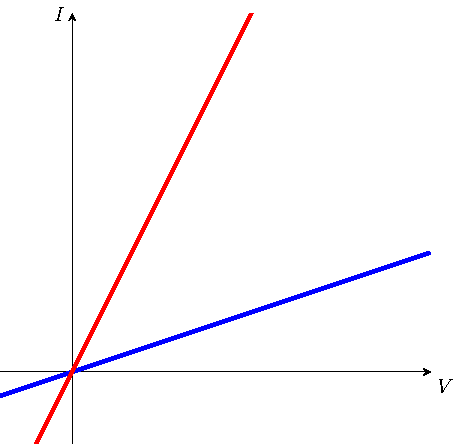
\includegraphics[width=.30\textwidth]{img/resistence-current}
    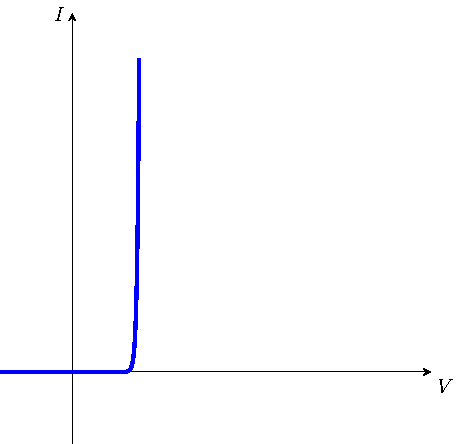
\includegraphics[width=.30\textwidth]{img/diode-current-graph}
\end{figure}

Possiamo osservare che il comportamento della corrente del diodo è completamente differente, e la legge di ohm ($\bar{J} = \sigma \bar{E}$) è valida in forma locale.

Analizziamo quindi più nel dettaglio la struttura dei materiali semiconduttori.

Gli elettroni dei materiali orbitano attorno ai rispettivi nuclei, perché si trovano in uno stato di equilibrio, dovuto alle forze coulombiane, tale per cui la somma complessiva delle cariche di un atomo è nulla.

Maggiore è l'orbita degli elettroni attorno al nucleo, maggiore è la velocità degli elettroni. Inoltre siccome la forza attrattiva dipende dal quadrato della distanza, più esterna è l'orbita, minore è la forza attrattiva che si manifesta.

All'ampiezza dell'orbita è quindi associato inversamente la forza attrattiva del nucleo, ed un'energia cinetica legata alla velocità di percorrenza.
\\
Possiamo quindi, gli elettroni interni ad un atomo generico in funzione dell'energia da essi posseduta, ottenendo un diagramma simile a quello in figura ..., distinta da diversi livelli

\begin{figure}[h]
    \centering
    \begin{tikzpicture}
        \draw[->] (0, 0) -- (0, 3)
            node[right]{$E$};

        \foreach \y in {.5, 1, ..., 2.5}
        {
            \draw (-3pt, \y) -- (+3pt, \y);
        }
    \end{tikzpicture}
\end{figure}

Ad ogni elettrone è dunque associato un livello sull'asse delle energie.
Per il principio di quantizzazione, dell'energia, non tutti i possibili livelli di energia sono possibili. L'asse quindi non è continua, ma quantizzata.

È importante notare che le orbite degli elettroni attorno agli atomi non sono descritte dalla meccanica classica, ma dalla meccanica quantistica, dove gli elettroni sono descritti attraverso forme sinusoidali.

Per questo motivo è possibile associare agli elettroni una lunghezza d'onda $\lambda$, dove nel caso di ipotesi stazionaria, è necessario che la circonferenza dell'orbita sia multiplo di $\lambda$.
\\
Questo spiega a grandi linee la presenza di valori permessi e proibiti sull'asse delle energie.

\subsubsection{Principio di esclusione di Pauli}
Ciascun livello energetico è occupabile al più da due elettroni (con spin opposto). In altre parole, il numero di elettroni che possono avere una certa distanza dal nucleo è finito.

Da questo è possibile dedurre che è possibile occupare interamente i livelli di energia.

Spostare corrente vuol dire spostare elettroni, cambiandone la velocità, quindi aumentandone l'energia cinetica, vincolata dai livelli di energia e dal principio di esclusione.

Per muovere un'elettrone quindi serve almeno l'energia per raggiungere il livello energetico libero più vicino.

Nel momento in cui due atomi diventino abbastanza vicini da interagire, quello che mi posso aspettare è che gli elettroni dei rispettivi atomi esercitino una forza repulsiva, con l'effetto di modificare l'orbita dei due elettroni.

Considerando quindi un unico diagramma energetico per il sistema dei due atomi, quello che ottengo è che i livelli non si sovrappongono ma si scostano leggermente, mantenendo comunque i principi di quantizzazione ed esclusione.

Generalizzando il discorso con un'interazione di $n$ atomi, otteniamo che ai precedenti livelli energetici, corrisponderà una moltitudine di livelli permessi, tra loro poco differenti, chiamata \textit{banda permessa}.
\\
I valori di energia tra due bande permesse, prendono il nome di \textit{banda proibita}.

È importante sottolineare che i valori interni alla banda permessa rispettano ancora il principio di esclusione e di quantizzazione, quindi è possibile che un'intera banda sia occupata da elettroni.

In condizione di quiete, gli elettroni tendono spontaneamente ad occupare i livelli con minore energia, quindi quelli più bassi.

La statistica di fermi indica un valore limite (\textit{Livello di Fermi}) che indica, in assenza di perturbazione, in termini probabilistici, tutti i livelli che sotto tale valore risultano occupati.

La posizione di questo livello diventa quindi fondamentale per indicare le condizioni di trasporto di carica del materiale.
Nel caso di materiali conduttori, il livello di fermi ricade internamente ad una banda permessa,
l'energia richiesta per spostare elettroni da livelli energetici occupati a livelli energetici liberi, è dipendente dalla loro distanza, quindi molto bassa.

Nel caso di materiali isolanti, il livello di fermi ricade all'interno di una banda proibita, l'energia sufficiente richiesta (energy gap) è quella per scavalcare l'intera banda proibita, quindi molto superiore al caso precedente.

I materiali isolanti sono dunque anch'essi soggetti a fenomeni di scarica elettrica.

\subsubsection{I semiconduttori}
Il semiconduttore ha una struttura simile a quella dell'isolante, quello che differisce è l'ampiezza del gap, richiedendo una quantità di energia bassa per effettuare il "salto" della banda proibita.
Se la quantità di energia ricevibile dalla temperatura dall'ambiente è pari o superiore al gap, diventa facile che elettroni passino da una banda energetica superiore.
Elettroni quindi nella banda permessa superiore, trovandola completamente vuota, richiedono a loro volta poca energia per muoversi da un livello energetico all'altro, fornendo al materiale caratteristiche di un conduttore.
Chiameremo quindi questa nuova banda, banda di conduzione, mentre chiameremo la vecchia banda, banda di valenza.

La banda di valenza, avendo anch'essa livelli svuotati da elettroni spostati in banda di conduzione, richiederà anch'essa poca energia per effettuare salti di gap interni alla banda.
La conducibilità elettrica aumenta quindi con la temperatura del circuito.

Riassumendo quindi, un semiconduttore il livello di fermi interseca una banda proibita, la cui ampiezza è sufficientemente piccola da essere probabile l'effetto di scavalcamento con la sola energia termica.
Il semiconduttore ha quindi "due" bande di conduzione.
\end{document}
